\subsection{System Monitoring} 

\begin{figure}[H]
    \centering
    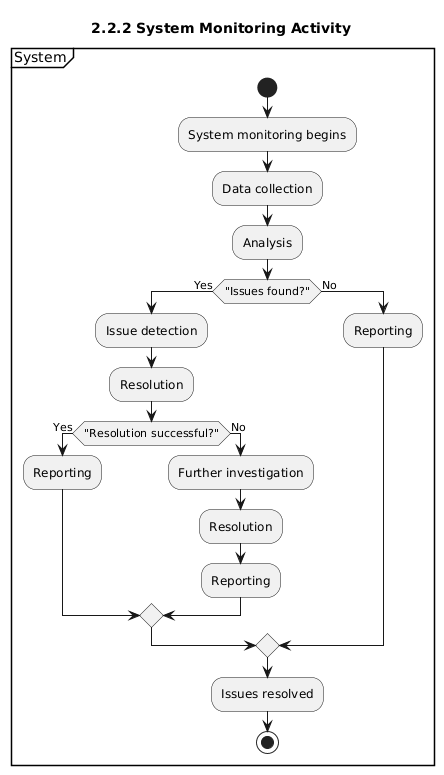
\includegraphics[width=0.7\textwidth]{graphics/chapter4/management/System_Monitoring_Activity.png} 
    \caption{System Monitoring Activity}
    \label{fig:Booking}
\end{figure}

\noindent \textbf{Description}

\begin{enumerate}
    \item \textbf{System:} Start monitoring and initialize processes.
    \item \textbf{System:} Collects operational and performance data.
    \item \textbf{System:} Performs data analysis to identify anomalies or irregularities.
    \item \textbf{Decision:} \textit{Issues found?} 
    \begin{itemize}
        \item Yes: Proceed to issue detection.
        \item No: Generate and send system report, then continue monitoring.
    \end{itemize}
    \item \textbf{System:} Detects and classifies the identified issues.
    \item \textbf{System:} Executes resolution procedures to address the detected issues.
    \item \textbf{Decision:} \textit{Resolution successful?}
    \begin{itemize}
        \item Yes: Generate resolution report and update monitoring records.
        \item No: Conduct further investigation and attempt another resolution cycle.
    \end{itemize}
    \item \textbf{System:} After successful resolution, updates system status and compiles a final report.
    \item \textbf{System:} Confirms that all issues have been resolved.
    \item \textbf{System:} Ends monitoring activity.
\end{enumerate}
